\section{Ablation study}\label{sec:ablation}

Table~\ref{tab:ablation} and Fig.~\ref{fig:ablation} report the effect of removing or modifying one
component of PI-PatchSurv at a time. The ablations of the physics branch, the survival head and the
synthetic data were run with three seeds, the chemistry prior and the tuned model with five, and the
remaining variants with one seed.

\begin{table*}[t]
\caption{Ablation of PI-PatchSurv. $\Delta$: reference minus variant on pooled AUPRC@24h (paired instance bootstrap, 95\,\% CI, Holm-corrected $p$).}\label{tab:ablation}
\scriptsize\setlength{\tabcolsep}{3pt}
\resizebox{\textwidth}{!}{\begin{tabular}{lccccccc}
\toprule
Variant & Seeds & AUPRC@24h & AUROC@24h & C-index & ECE & Hits/24 & $\Delta$ pooled AUPRC [CI], $p$ \\
\midrule
Full model (reference) & 5 & 0.644$\pm$0.055 & 0.794$\pm$0.018 & 0.802 & 0.234 & 5.8$\pm$2.9 & -- \\
$-$ physics branch & 3 & 0.581$\pm$0.036 & 0.718$\pm$0.002 & 0.730 & 0.295 & 7.0$\pm$3.0 & +0.068 [-0.05, +0.22], 1.00 \\
$-$ $\mathcal{L}_{\mathrm{mono}}$ & 1 & 0.664 & 0.771 & 0.750 & 0.243 & 4 & +0.005 [-0.04, +0.05], 1.00 \\
$-$ survival head (per-horizon BCE) & 3 & 0.682$\pm$0.030 & 0.842$\pm$0.045 & 0.778 & 0.155 & 3.0$\pm$1.7 & -0.231 [-0.39, -0.07], 0.27 \\
$-$ patching (patch length 1) & \multicolumn{7}{c}{not available} \\
patch 8, no overlap & 1 & 0.681 & 0.780 & 0.742 & 0.171 & 7 & -0.038 [-0.11, +0.04], 1.00 \\
$-$ synthetic training data & 3 & 0.654$\pm$0.032 & 0.911$\pm$0.001 & 0.754 & 0.247 & 9.3$\pm$2.5 & +0.217 [+0.08, +0.36], 0.07 \\
$+$ PHREEQC SI prior & 5 & 0.657$\pm$0.034 & 0.792$\pm$0.020 & 0.792 & 0.191 & 5.0$\pm$2.7 & -0.060 [-0.12, +0.01], 1.00 \\
Optuna-tuned & 5 & 0.596$\pm$0.093 & 0.746$\pm$0.076 & 0.765 & 0.285 & 5.6$\pm$2.9 & -0.009 [-0.13, +0.13], 1.00 \\
\bottomrule
\end{tabular}}
\end{table*}


\begin{figure}[t]
\centering
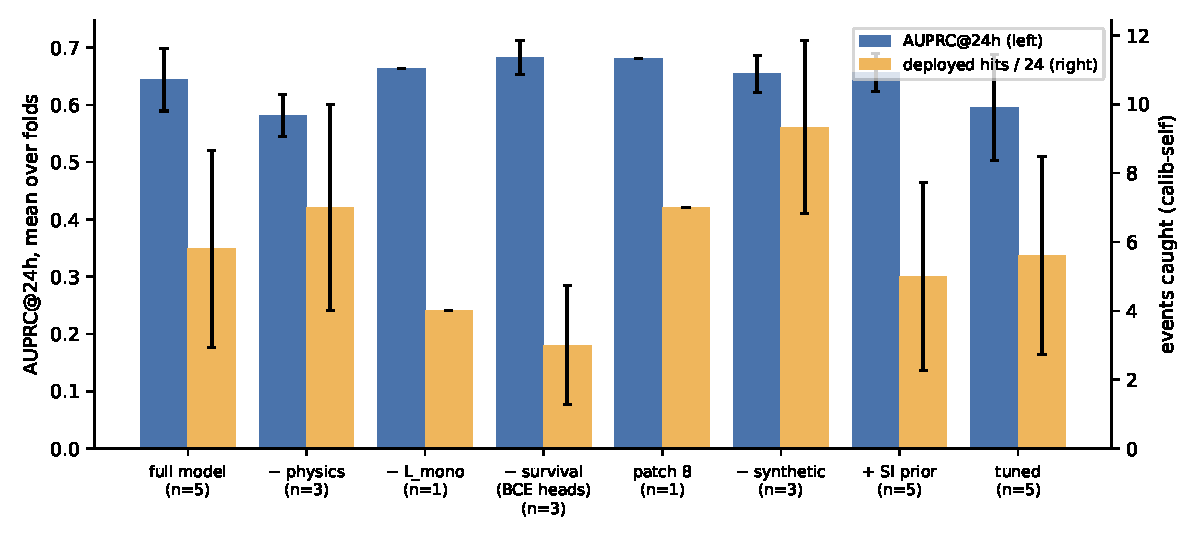
\includegraphics[width=0.7\textwidth]{figures/ablation_bars.pdf}
\caption{Ablation results: AUPRC@24h (left axis) and events caught with the deployed threshold (right axis).
Bars show the mean and whiskers one standard deviation over $n$ seeds}
\label{fig:ablation}
\end{figure}

The physics branch is the component with the clearest effect. Removing it lowers AUROC from
$0.794\pm0.018$ to $0.718\pm0.002$, the C-index from 0.80 to 0.73 and AUPRC from 0.644 to $0.581\pm0.036$,
and it worsens calibration (ECE from 0.23 to 0.30). The effect is consistent across seeds, which indicates
that the engineered restriction trends carry information that the patch encoder does not recover from 24
events alone.

Replacing the survival head by independent per-horizon classifiers gives a slightly higher AUPRC
($0.682\pm0.030$) and a higher pooled AUPRC (0.80 against 0.54), but fewer events caught under the deployed
threshold ($3.0\pm1.7$ against $5.8\pm2.9$), lower interval coverage (0.59 against 0.87) and risk curves
that are no longer guaranteed to increase with the horizon. Choosing between the two on the test wells would
amount to test-set selection, so the survival head is kept by design and the trade-off is reported.

Training on real instances only raises AUROC ($0.911\pm0.001$) and the number of deployed events
($9.3\pm2.5$), but pooled AUPRC falls from 0.54 to 0.34 and interval coverage from 0.87 to 0.45. The
simulated and hand-drawn instances therefore mainly make scores comparable across wells and calibrate the
time-to-event estimate, rather than improving the ranking within a well.

Removing patching (patch length 1, so that every minute becomes a token) lowers AUPRC from 0.726 to 0.628
and AUROC from 0.790 to 0.740 relative to the same seed of the full model, while raising the number of
tokens per channel from 44 to 360 and the training cost accordingly; a patch length of 8 without overlap
changes little. Removing the monotonicity loss is neutral in ranking but reduces the number of deployed
events. The PHREEQC saturation-index prior gives small, non-significant gains (AUPRC $0.657\pm0.034$, pooled
AUPRC 0.60, PICP 0.89); because the brines are a regional average rather than the wells' own water, this is
a lower bound on what chemistry can add. Finally, Optuna tuning on the calibration-well loss did not help
PI-PatchSurv ($0.596\pm0.093$), since the tuning objective is noisy when it rests on one small calibration
well.
